\documentclass[1p]{elsarticle_modified}
%\bibliographystyle{elsarticle-num}

%\usepackage[colorlinks]{hyperref}
%\usepackage{abbrmath_seonhwa} %\Abb, \Ascr, \Acal ,\Abf, \Afrak
\usepackage{amsfonts}
\usepackage{amssymb}
\usepackage{amsmath}
\usepackage{amsthm}
\usepackage{scalefnt}
\usepackage{amsbsy}
\usepackage{kotex}
\usepackage{caption}
\usepackage{subfig}
\usepackage{color}
\usepackage{graphicx}
\usepackage{xcolor} %% white, black, red, green, blue, cyan, magenta, yellow
\usepackage{float}
\usepackage{setspace}
\usepackage{hyperref}

\usepackage{tikz}
\usetikzlibrary{arrows}

\usepackage{multirow}
\usepackage{array} % fixed length table
\usepackage{hhline}

%%%%%%%%%%%%%%%%%%%%%
\makeatletter
\renewcommand*\env@matrix[1][\arraystretch]{%
	\edef\arraystretch{#1}%
	\hskip -\arraycolsep
	\let\@ifnextchar\new@ifnextchar
	\array{*\c@MaxMatrixCols c}}
\makeatother %https://tex.stackexchange.com/questions/14071/how-can-i-increase-the-line-spacing-in-a-matrix
%%%%%%%%%%%%%%%

\usepackage[normalem]{ulem}

\newcommand{\msout}[1]{\ifmmode\text{\sout{\ensuremath{#1}}}\else\sout{#1}\fi}
%SOURCE: \msout is \stkout macro in https://tex.stackexchange.com/questions/20609/strikeout-in-math-mode

\newcommand{\cancel}[1]{
	\ifmmode
	{\color{red}\msout{#1}}
	\else
	{\color{red}\sout{#1}}
	\fi
}

\newcommand{\add}[1]{
	{\color{blue}\uwave{#1}}
}

\newcommand{\replace}[2]{
	\ifmmode
	{\color{red}\msout{#1}}{\color{blue}\uwave{#2}}
	\else
	{\color{red}\sout{#1}}{\color{blue}\uwave{#2}}
	\fi
}

\newcommand{\Sol}{\mathcal{S}} %segment
\newcommand{\D}{D} %diagram
\newcommand{\A}{\mathcal{A}} %arc


%%%%%%%%%%%%%%%%%%%%%%%%%%%%%5 test

\def\sl{\operatorname{\textup{SL}}(2,\Cbb)}
\def\psl{\operatorname{\textup{PSL}}(2,\Cbb)}
\def\quan{\mkern 1mu \triangleright \mkern 1mu}

\theoremstyle{definition}
\newtheorem{thm}{Theorem}[section]
\newtheorem{prop}[thm]{Proposition}
\newtheorem{lem}[thm]{Lemma}
\newtheorem{ques}[thm]{Question}
\newtheorem{cor}[thm]{Corollary}
\newtheorem{defn}[thm]{Definition}
\newtheorem{exam}[thm]{Example}
\newtheorem{rmk}[thm]{Remark}
\newtheorem{alg}[thm]{Algorithm}

\newcommand{\I}{\sqrt{-1}}
\begin{document}

%\begin{frontmatter}
%
%\title{Boundary parabolic representations of knots up to 8 crossings}
%
%%% Group authors per affiliation:
%\author{Yunhi Cho} 
%\address{Department of Mathematics, University of Seoul, Seoul, Korea}
%\ead{yhcho@uos.ac.kr}
%
%
%\author{Seonhwa Kim} %\fnref{s_kim}}
%\address{Center for Geometry and Physics, Institute for Basic Science, Pohang, 37673, Korea}
%\ead{ryeona17@ibs.re.kr}
%
%\author{Hyuk Kim}
%\address{Department of Mathematical Sciences, Seoul National University, Seoul 08826, Korea}
%\ead{hyukkim@snu.ac.kr}
%
%\author{Seokbeom Yoon}
%\address{Department of Mathematical Sciences, Seoul National University, Seoul, 08826,  Korea}
%\ead{sbyoon15@snu.ac.kr}
%
%\begin{abstract}
%We find all boundary parabolic representation of knots up to 8 crossings.
%
%\end{abstract}
%\begin{keyword}
%    \MSC[2010] 57M25 
%\end{keyword}
%
%\end{frontmatter}

%\linenumbers
%\tableofcontents
%
\newcommand\colored[1]{\textcolor{white}{\rule[-0.35ex]{0.8em}{1.4ex}}\kern-0.8em\color{red} #1}%
%\newcommand\colored[1]{\textcolor{white}{ #1}\kern-2.17ex	\textcolor{white}{ #1}\kern-1.81ex	\textcolor{white}{ #1}\kern-2.15ex\color{red}#1	}

{\Large $\underline{12n_{0012}~(K12n_{0012})}$}

\setlength{\tabcolsep}{10pt}
\renewcommand{\arraystretch}{1.6}
\vspace{1cm}\begin{tabular}{m{100pt}>{\centering\arraybackslash}m{274pt}}
\multirow{5}{120pt}{
	\centering
	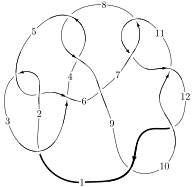
\includegraphics[width=112pt]{../../../GIT/diagram.site/Diagrams/png/2101_12n_0012.png}\\
\ \ \ A knot diagram\footnotemark}&
\allowdisplaybreaks
\textbf{Linearized knot diagam} \\
\cline{2-2}
 &
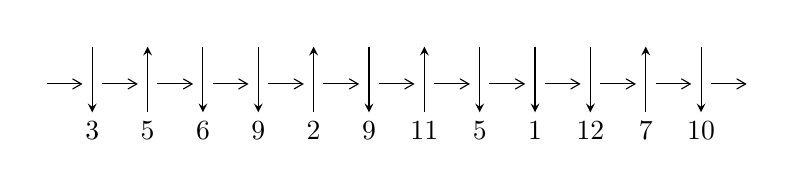
\begin{tikzpicture}[x=20pt, y=17pt]
	% nodes
	\node (C0) at (0, 0) {};
	\node (C1) at (1, 0) {};
	\node (C1U) at (1, +1) {};
	\node (C1D) at (1, -1) {3};

	\node (C2) at (2, 0) {};
	\node (C2U) at (2, +1) {};
	\node (C2D) at (2, -1) {5};

	\node (C3) at (3, 0) {};
	\node (C3U) at (3, +1) {};
	\node (C3D) at (3, -1) {6};

	\node (C4) at (4, 0) {};
	\node (C4U) at (4, +1) {};
	\node (C4D) at (4, -1) {9};

	\node (C5) at (5, 0) {};
	\node (C5U) at (5, +1) {};
	\node (C5D) at (5, -1) {2};

	\node (C6) at (6, 0) {};
	\node (C6U) at (6, +1) {};
	\node (C6D) at (6, -1) {9};

	\node (C7) at (7, 0) {};
	\node (C7U) at (7, +1) {};
	\node (C7D) at (7, -1) {11};

	\node (C8) at (8, 0) {};
	\node (C8U) at (8, +1) {};
	\node (C8D) at (8, -1) {5};

	\node (C9) at (9, 0) {};
	\node (C9U) at (9, +1) {};
	\node (C9D) at (9, -1) {1};

	\node (C10) at (10, 0) {};
	\node (C10U) at (10, +1) {};
	\node (C10D) at (10, -1) {12};

	\node (C11) at (11, 0) {};
	\node (C11U) at (11, +1) {};
	\node (C11D) at (11, -1) {7};

	\node (C12) at (12, 0) {};
	\node (C12U) at (12, +1) {};
	\node (C12D) at (12, -1) {10};
	\node (C13) at (13, 0) {};

	% arrows
	\draw[->,>={angle 60}]
	(C0) edge (C1) (C1) edge (C2) (C2) edge (C3) (C3) edge (C4) (C4) edge (C5) (C5) edge (C6) (C6) edge (C7) (C7) edge (C8) (C8) edge (C9) (C9) edge (C10) (C10) edge (C11) (C11) edge (C12) (C12) edge (C13) ;	\draw[->,>=stealth]
	(C1U) edge (C1D) (C2D) edge (C2U) (C3U) edge (C3D) (C4U) edge (C4D) (C5D) edge (C5U) (C6U) edge (C6D) (C7D) edge (C7U) (C8U) edge (C8D) (C9U) edge (C9D) (C10U) edge (C10D) (C11D) edge (C11U) (C12U) edge (C12D) ;
	\end{tikzpicture} \\
\hhline{~~} \\& 
\textbf{Solving Sequence} \\ \cline{2-2} 
 &
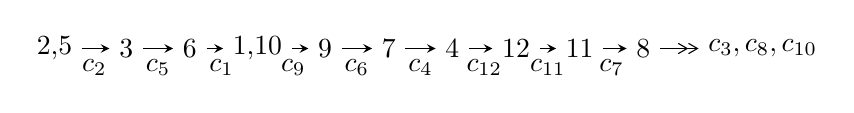
\begin{tikzpicture}[x=23pt, y=7pt]
	% node
	\node (A0) at (-1/8, 0) {2,5};
	\node (A1) at (1, 0) {3};
	\node (A2) at (2, 0) {6};
	\node (A3) at (49/16, 0) {1,10};
	\node (A4) at (33/8, 0) {9};
	\node (A5) at (41/8, 0) {7};
	\node (A6) at (49/8, 0) {4};
	\node (A7) at (57/8, 0) {12};
	\node (A8) at (65/8, 0) {11};
	\node (A9) at (73/8, 0) {8};
	\node (C1) at (1/2, -1) {$c_{2}$};
	\node (C2) at (3/2, -1) {$c_{5}$};
	\node (C3) at (5/2, -1) {$c_{1}$};
	\node (C4) at (29/8, -1) {$c_{9}$};
	\node (C5) at (37/8, -1) {$c_{6}$};
	\node (C6) at (45/8, -1) {$c_{4}$};
	\node (C7) at (53/8, -1) {$c_{12}$};
	\node (C8) at (61/8, -1) {$c_{11}$};
	\node (C9) at (69/8, -1) {$c_{7}$};
	\node (A10) at (11, 0) {$c_{3},c_{8},c_{10}$};

	% edge
	\draw[->,>=stealth]	
	(A0) edge (A1) (A1) edge (A2) (A2) edge (A3) (A3) edge (A4) (A4) edge (A5) (A5) edge (A6) (A6) edge (A7) (A7) edge (A8) (A8) edge (A9) ;
	\draw[->>,>={angle 60}]	
	(A9) edge (A10);
\end{tikzpicture} \\ 

\end{tabular} \\

\footnotetext{
The image of knot diagram is generated by the software ``\textbf{Draw programme}" developed by Andrew Bartholomew(\url{http://www.layer8.co.uk/maths/draw/index.htm\#Running-draw}), where we modified some parts for our purpose(\url{https://github.com/CATsTAILs/LinksPainter}).
}\phantom \\ \newline 
\centering \textbf{Ideals for irreducible components\footnotemark of $X_{\text{par}}$} 
 
\begin{align*}
I^u_{1}&=\langle 
-39 u^{46}+220 u^{45}+\cdots+8 b-74,\;-3 u^{46}+13 u^{45}+\cdots+8 a-17,\;u^{47}-5 u^{46}+\cdots+2 u-1\rangle \\
I^u_{2}&=\langle 
a u+b- a,\;a^4+a^3 u-3 a^2 u-3 a^2+2 a+u,\;u^2+u+1\rangle \\
\\
\end{align*}
\raggedright * 2 irreducible components of $\dim_{\mathbb{C}}=0$, with total 55 representations.\\
\footnotetext{All coefficients of polynomials are rational numbers. But the coefficients are sometimes approximated in decimal forms when there is not enough margin.}
\newpage
\renewcommand{\arraystretch}{1}
\centering \section*{I. $I^u_{1}= \langle -39 u^{46}+220 u^{45}+\cdots+8 b-74,\;-3 u^{46}+13 u^{45}+\cdots+8 a-17,\;u^{47}-5 u^{46}+\cdots+2 u-1 \rangle$}
\flushleft \textbf{(i) Arc colorings}\\
\begin{tabular}{m{7pt} m{180pt} m{7pt} m{180pt} }
\flushright $a_{2}=$&$\begin{pmatrix}1\\0\end{pmatrix}$ \\
\flushright $a_{5}=$&$\begin{pmatrix}0\\u\end{pmatrix}$ \\
\flushright $a_{3}=$&$\begin{pmatrix}1\\- u^2\end{pmatrix}$ \\
\flushright $a_{6}=$&$\begin{pmatrix}u\\u\end{pmatrix}$ \\
\flushright $a_{1}=$&$\begin{pmatrix}u^2+1\\- u^4\end{pmatrix}$ \\
\flushright $a_{10}=$&$\begin{pmatrix}\frac{3}{8} u^{46}-\frac{13}{8} u^{45}+\cdots-\frac{25}{4} u+\frac{17}{8}\\\frac{39}{8} u^{46}-\frac{55}{2} u^{45}+\cdots-\frac{155}{8} u+\frac{37}{4}\end{pmatrix}$ \\
\flushright $a_{9}=$&$\begin{pmatrix}-\frac{9}{4} u^{46}+\frac{39}{4} u^{45}+\cdots-5 u+\frac{11}{4}\\\frac{5}{4} u^{46}-\frac{89}{8} u^{45}+\cdots-\frac{105}{8} u+\frac{55}{8}\end{pmatrix}$ \\
\flushright $a_{7}=$&$\begin{pmatrix}- u^2-1\\-\frac{1}{8} u^{46}+\frac{5}{8} u^{45}+\cdots+\frac{9}{4} u-\frac{1}{8}\end{pmatrix}$ \\
\flushright $a_{4}=$&$\begin{pmatrix}u^4+u^2+1\\u^4\end{pmatrix}$ \\
\flushright $a_{12}=$&$\begin{pmatrix}\frac{1}{8} u^{46}-\frac{1}{2} u^{45}+\cdots+\frac{7}{8} u+2\\\frac{1}{4} u^{46}-\frac{9}{8} u^{45}+\cdots-\frac{11}{8} u+\frac{1}{8}\end{pmatrix}$ \\
\flushright $a_{11}=$&$\begin{pmatrix}\frac{7}{4} u^{46}-\frac{31}{4} u^{45}+\cdots-\frac{9}{2} u+\frac{5}{2}\\-2 u^{46}+\frac{145}{8} u^{45}+\cdots+\frac{121}{8} u-\frac{93}{8}\end{pmatrix}$ \\
\flushright $a_{8}=$&$\begin{pmatrix}\frac{9}{4} u^{46}-\frac{39}{4} u^{45}+\cdots+5 u-\frac{11}{4}\\\frac{1}{2} u^{46}+\frac{41}{8} u^{45}+\cdots+\frac{111}{8} u-\frac{67}{8}\end{pmatrix}$\\&\end{tabular}
\flushleft \textbf{(ii) Obstruction class $= -1$}\\~\\
\flushleft \textbf{(iii) Cusp Shapes $= \frac{3}{8} u^{46}+6 u^{45}+\cdots+\frac{335}{8} u-\frac{31}{2}$}\\~\\
\newpage\renewcommand{\arraystretch}{1}
\flushleft \textbf{(iv) u-Polynomials at the component}\newline \\
\begin{tabular}{m{50pt}|m{274pt}}
Crossings & \hspace{64pt}u-Polynomials at each crossing \\
\hline $$\begin{aligned}c_{1}\end{aligned}$$&$\begin{aligned}
&u^{47}+27 u^{46}+\cdots-40 u-1
\end{aligned}$\\
\hline $$\begin{aligned}c_{2},c_{5}\end{aligned}$$&$\begin{aligned}
&u^{47}+5 u^{46}+\cdots+2 u+1
\end{aligned}$\\
\hline $$\begin{aligned}c_{3}\end{aligned}$$&$\begin{aligned}
&u^{47}-5 u^{46}+\cdots-12 u+1
\end{aligned}$\\
\hline $$\begin{aligned}c_{4},c_{8}\end{aligned}$$&$\begin{aligned}
&u^{47}+u^{46}+\cdots+640 u+256
\end{aligned}$\\
\hline $$\begin{aligned}c_{6}\end{aligned}$$&$\begin{aligned}
&u^{47}-3 u^{46}+\cdots-4 u+1
\end{aligned}$\\
\hline $$\begin{aligned}c_{7},c_{11}\end{aligned}$$&$\begin{aligned}
&u^{47}-3 u^{46}+\cdots-2 u+1
\end{aligned}$\\
\hline $$\begin{aligned}c_{9},c_{10},c_{12}\end{aligned}$$&$\begin{aligned}
&u^{47}+13 u^{46}+\cdots-16 u-1
\end{aligned}$\\
\hline
\end{tabular}\\~\\
\newpage\renewcommand{\arraystretch}{1}
\flushleft \textbf{(v) Riley Polynomials at the component}\newline \\
\begin{tabular}{m{50pt}|m{274pt}}
Crossings & \hspace{64pt}Riley Polynomials at each crossing \\
\hline $$\begin{aligned}c_{1}\end{aligned}$$&$\begin{aligned}
&y^{47}-9 y^{46}+\cdots+512 y-1
\end{aligned}$\\
\hline $$\begin{aligned}c_{2},c_{5}\end{aligned}$$&$\begin{aligned}
&y^{47}+27 y^{46}+\cdots-40 y-1
\end{aligned}$\\
\hline $$\begin{aligned}c_{3}\end{aligned}$$&$\begin{aligned}
&y^{47}-45 y^{46}+\cdots-152 y-1
\end{aligned}$\\
\hline $$\begin{aligned}c_{4},c_{8}\end{aligned}$$&$\begin{aligned}
&y^{47}-45 y^{46}+\cdots+638976 y-65536
\end{aligned}$\\
\hline $$\begin{aligned}c_{6}\end{aligned}$$&$\begin{aligned}
&y^{47}-55 y^{46}+\cdots-16 y-1
\end{aligned}$\\
\hline $$\begin{aligned}c_{7},c_{11}\end{aligned}$$&$\begin{aligned}
&y^{47}+13 y^{46}+\cdots-16 y-1
\end{aligned}$\\
\hline $$\begin{aligned}c_{9},c_{10},c_{12}\end{aligned}$$&$\begin{aligned}
&y^{47}+45 y^{46}+\cdots-8 y-1
\end{aligned}$\\
\hline
\end{tabular}\\~\\
\newpage\flushleft \textbf{(vi) Complex Volumes and Cusp Shapes}
$$\begin{array}{c|c|c}  
\text{Solutions to }I^u_{1}& \I (\text{vol} + \sqrt{-1}CS) & \text{Cusp shape}\\
 \hline 
\begin{aligned}
u &= \phantom{-}0.026441 + 0.959622 I \\
a &= -0.602286 + 0.667947 I \\
b &= -0.28964 + 2.11687 I\end{aligned}
 & -1.66847 + 2.07597 I & -8.19599 - 3.58729 I \\ \hline\begin{aligned}
u &= \phantom{-}0.026441 - 0.959622 I \\
a &= -0.602286 - 0.667947 I \\
b &= -0.28964 - 2.11687 I\end{aligned}
 & -1.66847 - 2.07597 I & -8.19599 + 3.58729 I \\ \hline\begin{aligned}
u &= \phantom{-}0.925280 + 0.194352 I \\
a &= -1.48851 + 2.82129 I \\
b &= \phantom{-}0.86927 - 1.38303 I\end{aligned}
 & \phantom{-}0.19889 - 8.32605 I & -2.17091 + 5.11912 I \\ \hline\begin{aligned}
u &= \phantom{-}0.925280 - 0.194352 I \\
a &= -1.48851 - 2.82129 I \\
b &= \phantom{-}0.86927 + 1.38303 I\end{aligned}
 & \phantom{-}0.19889 + 8.32605 I & -2.17091 - 5.11912 I \\ \hline\begin{aligned}
u &= \phantom{-}0.933825 + 0.065187 I \\
a &= \phantom{-}0.120868 + 1.140740 I \\
b &= -0.501416 - 0.737782 I\end{aligned}
 & -6.55195 - 3.23257 I & -7.12321 + 3.54877 I \\ \hline\begin{aligned}
u &= \phantom{-}0.933825 - 0.065187 I \\
a &= \phantom{-}0.120868 - 1.140740 I \\
b &= -0.501416 + 0.737782 I\end{aligned}
 & -6.55195 + 3.23257 I & -7.12321 - 3.54877 I \\ \hline\begin{aligned}
u &= -0.733010 + 0.802557 I \\
a &= -2.03414 - 2.16959 I \\
b &= -0.82061 - 2.32750 I\end{aligned}
 & \phantom{-}4.57748 + 0.17561 I & -4.00000 + 0. I\phantom{ +0.000000I} \\ \hline\begin{aligned}
u &= -0.733010 - 0.802557 I \\
a &= -2.03414 + 2.16959 I \\
b &= -0.82061 + 2.32750 I\end{aligned}
 & \phantom{-}4.57748 - 0.17561 I & -4.00000 + 0. I\phantom{ +0.000000I} \\ \hline\begin{aligned}
u &= -0.580519 + 0.922395 I \\
a &= \phantom{-}1.018240 - 0.170806 I \\
b &= \phantom{-}1.221000 - 0.367778 I\end{aligned}
 & -0.75821 - 2.95186 I & -10.26739 + 0. I\phantom{ +0.000000I} \\ \hline\begin{aligned}
u &= -0.580519 - 0.922395 I \\
a &= \phantom{-}1.018240 + 0.170806 I \\
b &= \phantom{-}1.221000 + 0.367778 I\end{aligned}
 & -0.75821 + 2.95186 I & -10.26739 + 0. I\phantom{ +0.000000I}\\
 \hline 
 \end{array}$$\newpage$$\begin{array}{c|c|c}  
\text{Solutions to }I^u_{1}& \I (\text{vol} + \sqrt{-1}CS) & \text{Cusp shape}\\
 \hline 
\begin{aligned}
u &= \phantom{-}0.886435 + 0.192716 I \\
a &= \phantom{-}1.79497 - 2.22924 I \\
b &= -0.835270 + 0.957471 I\end{aligned}
 & \phantom{-}0.91039 - 2.22540 I & -1.015220 + 0.333993 I \\ \hline\begin{aligned}
u &= \phantom{-}0.886435 - 0.192716 I \\
a &= \phantom{-}1.79497 + 2.22924 I \\
b &= -0.835270 - 0.957471 I\end{aligned}
 & \phantom{-}0.91039 + 2.22540 I & -1.015220 - 0.333993 I \\ \hline\begin{aligned}
u &= -0.232117 + 1.073970 I \\
a &= -0.764740 + 0.107154 I \\
b &= -0.930392 - 0.122544 I\end{aligned}
 & -3.32956 - 2.69471 I & -11.16965 + 4.64357 I \\ \hline\begin{aligned}
u &= -0.232117 - 1.073970 I \\
a &= -0.764740 - 0.107154 I \\
b &= -0.930392 + 0.122544 I\end{aligned}
 & -3.32956 + 2.69471 I & -11.16965 - 4.64357 I \\ \hline\begin{aligned}
u &= -0.732051 + 0.844151 I \\
a &= \phantom{-}2.53321 + 1.61725 I \\
b &= \phantom{-}1.64457 + 2.36743 I\end{aligned}
 & \phantom{-}4.45822 - 5.68770 I & \phantom{-0.000000 -}0. + 5.85551 I \\ \hline\begin{aligned}
u &= -0.732051 - 0.844151 I \\
a &= \phantom{-}2.53321 - 1.61725 I \\
b &= \phantom{-}1.64457 - 2.36743 I\end{aligned}
 & \phantom{-}4.45822 + 5.68770 I & \phantom{-0.000000 } 0. - 5.85551 I \\ \hline\begin{aligned}
u &= \phantom{-}0.278391 + 0.834871 I \\
a &= \phantom{-}0.195597 - 0.017136 I \\
b &= \phantom{-}2.04050 + 2.00587 I\end{aligned}
 & \phantom{-}6.29656 + 4.54704 I & -5.32988 - 0.19475 I \\ \hline\begin{aligned}
u &= \phantom{-}0.278391 - 0.834871 I \\
a &= \phantom{-}0.195597 + 0.017136 I \\
b &= \phantom{-}2.04050 - 2.00587 I\end{aligned}
 & \phantom{-}6.29656 - 4.54704 I & -5.32988 + 0.19475 I \\ \hline\begin{aligned}
u &= -0.468535 + 0.741736 I \\
a &= \phantom{-}0.169080 - 0.871234 I \\
b &= -0.179453 - 0.614868 I\end{aligned}
 & -0.10080 - 1.41741 I & -3.72542 + 5.86093 I \\ \hline\begin{aligned}
u &= -0.468535 - 0.741736 I \\
a &= \phantom{-}0.169080 + 0.871234 I \\
b &= -0.179453 + 0.614868 I\end{aligned}
 & -0.10080 + 1.41741 I & -3.72542 - 5.86093 I\\
 \hline 
 \end{array}$$\newpage$$\begin{array}{c|c|c}  
\text{Solutions to }I^u_{1}& \I (\text{vol} + \sqrt{-1}CS) & \text{Cusp shape}\\
 \hline 
\begin{aligned}
u &= \phantom{-}0.856224\phantom{ +0.000000I} \\
a &= \phantom{-}0.798257\phantom{ +0.000000I} \\
b &= \phantom{-}0.0288409\phantom{ +0.000000I}\end{aligned}
 & -3.24343\phantom{ +0.000000I} & -1.24520\phantom{ +0.000000I} \\ \hline\begin{aligned}
u &= \phantom{-}0.277747 + 0.799964 I \\
a &= -0.031950 + 0.201535 I \\
b &= -1.99709 - 1.62792 I\end{aligned}
 & \phantom{-}6.39944 - 1.84713 I & -4.44776 + 5.17555 I \\ \hline\begin{aligned}
u &= \phantom{-}0.277747 - 0.799964 I \\
a &= -0.031950 - 0.201535 I \\
b &= -1.99709 + 1.62792 I\end{aligned}
 & \phantom{-}6.39944 + 1.84713 I & -4.44776 - 5.17555 I \\ \hline\begin{aligned}
u &= -0.215715 + 0.766929 I \\
a &= \phantom{-}0.623937 - 0.580705 I \\
b &= -0.040575 - 0.820520 I\end{aligned}
 & -0.273553 - 1.319440 I & -1.87412 + 4.02854 I \\ \hline\begin{aligned}
u &= -0.215715 - 0.766929 I \\
a &= \phantom{-}0.623937 + 0.580705 I \\
b &= -0.040575 + 0.820520 I\end{aligned}
 & -0.273553 + 1.319440 I & -1.87412 - 4.02854 I \\ \hline\begin{aligned}
u &= -0.443222 + 1.123720 I \\
a &= -0.306235 - 0.216455 I \\
b &= -1.89659 - 0.62970 I\end{aligned}
 & \phantom{-}2.20908 - 1.05804 I & \phantom{-0.000000 } 0 \\ \hline\begin{aligned}
u &= -0.443222 - 1.123720 I \\
a &= -0.306235 + 0.216455 I \\
b &= -1.89659 + 0.62970 I\end{aligned}
 & \phantom{-}2.20908 + 1.05804 I & \phantom{-0.000000 } 0 \\ \hline\begin{aligned}
u &= -0.403667 + 1.155110 I \\
a &= \phantom{-}0.258478 - 0.232515 I \\
b &= \phantom{-}2.08868 - 0.64022 I\end{aligned}
 & \phantom{-}1.85423 - 6.77428 I & \phantom{-0.000000 } 0 \\ \hline\begin{aligned}
u &= -0.403667 - 1.155110 I \\
a &= \phantom{-}0.258478 + 0.232515 I \\
b &= \phantom{-}2.08868 + 0.64022 I\end{aligned}
 & \phantom{-}1.85423 + 6.77428 I & \phantom{-0.000000 } 0 \\ \hline\begin{aligned}
u &= \phantom{-}0.348879 + 1.251500 I \\
a &= \phantom{-}0.68603 + 1.45153 I \\
b &= \phantom{-}2.92026 + 3.49905 I\end{aligned}
 & -3.64593 + 1.84085 I & \phantom{-0.000000 } 0\\
 \hline 
 \end{array}$$\newpage$$\begin{array}{c|c|c}  
\text{Solutions to }I^u_{1}& \I (\text{vol} + \sqrt{-1}CS) & \text{Cusp shape}\\
 \hline 
\begin{aligned}
u &= \phantom{-}0.348879 - 1.251500 I \\
a &= \phantom{-}0.68603 - 1.45153 I \\
b &= \phantom{-}2.92026 - 3.49905 I\end{aligned}
 & -3.64593 - 1.84085 I & \phantom{-0.000000 } 0 \\ \hline\begin{aligned}
u &= \phantom{-}0.467749 + 1.244070 I \\
a &= -0.178953 + 0.487783 I \\
b &= -0.489450 + 0.885522 I\end{aligned}
 & -6.97041 + 4.72417 I & \phantom{-0.000000 } 0 \\ \hline\begin{aligned}
u &= \phantom{-}0.467749 - 1.244070 I \\
a &= -0.178953 - 0.487783 I \\
b &= -0.489450 - 0.885522 I\end{aligned}
 & -6.97041 - 4.72417 I & \phantom{-0.000000 } 0 \\ \hline\begin{aligned}
u &= \phantom{-}0.339549 + 1.291160 I \\
a &= -1.09098 - 1.58824 I \\
b &= -4.42832 - 3.64735 I\end{aligned}
 & -4.58314 - 4.07496 I & \phantom{-0.000000 } 0 \\ \hline\begin{aligned}
u &= \phantom{-}0.339549 - 1.291160 I \\
a &= -1.09098 + 1.58824 I \\
b &= -4.42832 + 3.64735 I\end{aligned}
 & -4.58314 + 4.07496 I & \phantom{-0.000000 } 0 \\ \hline\begin{aligned}
u &= \phantom{-}0.552325 + 1.220220 I \\
a &= -1.88083 + 0.66995 I \\
b &= -4.90066 + 2.68102 I\end{aligned}
 & -2.19262 + 7.48494 I & \phantom{-0.000000 } 0 \\ \hline\begin{aligned}
u &= \phantom{-}0.552325 - 1.220220 I \\
a &= -1.88083 - 0.66995 I \\
b &= -4.90066 - 2.68102 I\end{aligned}
 & -2.19262 - 7.48494 I & \phantom{-0.000000 } 0 \\ \hline\begin{aligned}
u &= -0.643389 + 0.042276 I \\
a &= \phantom{-}0.307917 + 0.399006 I \\
b &= -0.124452 - 1.032220 I\end{aligned}
 & \phantom{-}5.17223 - 2.96380 I & \phantom{-}1.27670 + 2.94526 I \\ \hline\begin{aligned}
u &= -0.643389 - 0.042276 I \\
a &= \phantom{-}0.307917 - 0.399006 I \\
b &= -0.124452 + 1.032220 I\end{aligned}
 & \phantom{-}5.17223 + 2.96380 I & \phantom{-}1.27670 - 2.94526 I \\ \hline\begin{aligned}
u &= \phantom{-}0.564900 + 1.232880 I \\
a &= \phantom{-}2.21676 - 0.36369 I \\
b &= \phantom{-}6.02517 - 2.25245 I\end{aligned}
 & -2.95715 + 13.73810 I & \phantom{-0.000000 } 0\\
 \hline 
 \end{array}$$\newpage$$\begin{array}{c|c|c}  
\text{Solutions to }I^u_{1}& \I (\text{vol} + \sqrt{-1}CS) & \text{Cusp shape}\\
 \hline 
\begin{aligned}
u &= \phantom{-}0.564900 - 1.232880 I \\
a &= \phantom{-}2.21676 + 0.36369 I \\
b &= \phantom{-}6.02517 + 2.25245 I\end{aligned}
 & -2.95715 - 13.73810 I & \phantom{-0.000000 } 0 \\ \hline\begin{aligned}
u &= \phantom{-}0.435963 + 1.291860 I \\
a &= -0.743213 - 0.242847 I \\
b &= -2.18896 + 0.57747 I\end{aligned}
 & -10.77840 + 1.57100 I & \phantom{-0.000000 } 0 \\ \hline\begin{aligned}
u &= \phantom{-}0.435963 - 1.291860 I \\
a &= -0.743213 + 0.242847 I \\
b &= -2.18896 - 0.57747 I\end{aligned}
 & -10.77840 - 1.57100 I & \phantom{-0.000000 } 0 \\ \hline\begin{aligned}
u &= \phantom{-}0.509079 + 1.270360 I \\
a &= \phantom{-}0.692225 + 0.316516 I \\
b &= \phantom{-}2.63689 + 1.02049 I\end{aligned}
 & -10.24110 + 8.40839 I & \phantom{-0.000000 } 0 \\ \hline\begin{aligned}
u &= \phantom{-}0.509079 - 1.270360 I \\
a &= \phantom{-}0.692225 - 0.316516 I \\
b &= \phantom{-}2.63689 - 1.02049 I\end{aligned}
 & -10.24110 - 8.40839 I & \phantom{-0.000000 } 0 \\ \hline\begin{aligned}
u &= -0.022449 + 0.247534 I \\
a &= \phantom{-}1.60540 - 1.10956 I \\
b &= -0.337887 - 0.386120 I\end{aligned}
 & -0.255033 - 1.107400 I & -3.72059 + 6.13127 I \\ \hline\begin{aligned}
u &= -0.022449 - 0.247534 I \\
a &= \phantom{-}1.60540 + 1.10956 I \\
b &= -0.337887 + 0.386120 I\end{aligned}
 & -0.255033 + 1.107400 I & -3.72059 - 6.13127 I\\
 \hline 
 \end{array}$$\newpage\newpage\renewcommand{\arraystretch}{1}
\centering \section*{II. $I^u_{2}= \langle a u+b- a,\;a^4+a^3 u-3 a^2 u-3 a^2+2 a+u,\;u^2+u+1 \rangle$}
\flushleft \textbf{(i) Arc colorings}\\
\begin{tabular}{m{7pt} m{180pt} m{7pt} m{180pt} }
\flushright $a_{2}=$&$\begin{pmatrix}1\\0\end{pmatrix}$ \\
\flushright $a_{5}=$&$\begin{pmatrix}0\\u\end{pmatrix}$ \\
\flushright $a_{3}=$&$\begin{pmatrix}1\\u+1\end{pmatrix}$ \\
\flushright $a_{6}=$&$\begin{pmatrix}u\\u\end{pmatrix}$ \\
\flushright $a_{1}=$&$\begin{pmatrix}- u\\- u\end{pmatrix}$ \\
\flushright $a_{10}=$&$\begin{pmatrix}a\\- a u+a\end{pmatrix}$ \\
\flushright $a_{9}=$&$\begin{pmatrix}0\\- a u\end{pmatrix}$ \\
\flushright $a_{7}=$&$\begin{pmatrix}u\\a^2+u\end{pmatrix}$ \\
\flushright $a_{4}=$&$\begin{pmatrix}0\\u\end{pmatrix}$ \\
\flushright $a_{12}=$&$\begin{pmatrix}a^2 u+a^2- u\\a^2 u+2 a^2- u\end{pmatrix}$ \\
\flushright $a_{11}=$&$\begin{pmatrix}a^3 u+2 a\\2 a^3 u+a^3- a u+2 a\end{pmatrix}$ \\
\flushright $a_{8}=$&$\begin{pmatrix}0\\- a u\end{pmatrix}$\\&\end{tabular}
\flushleft \textbf{(ii) Obstruction class $= 1$}\\~\\
\flushleft \textbf{(iii) Cusp Shapes $= 2 a^3 u-4 a^3-5 a^2 u+12 a u+17 a+5 u-6$}\\~\\
\newpage\renewcommand{\arraystretch}{1}
\flushleft \textbf{(iv) u-Polynomials at the component}\newline \\
\begin{tabular}{m{50pt}|m{274pt}}
Crossings & \hspace{64pt}u-Polynomials at each crossing \\
\hline $$\begin{aligned}c_{1},c_{3},c_{5}\end{aligned}$$&$\begin{aligned}
&(u^2- u+1)^4
\end{aligned}$\\
\hline $$\begin{aligned}c_{2}\end{aligned}$$&$\begin{aligned}
&(u^2+u+1)^4
\end{aligned}$\\
\hline $$\begin{aligned}c_{4},c_{8}\end{aligned}$$&$\begin{aligned}
&u^8
\end{aligned}$\\
\hline $$\begin{aligned}c_{6},c_{9},c_{10}\end{aligned}$$&$\begin{aligned}
&(u^4- u^3+3 u^2-2 u+1)^2
\end{aligned}$\\
\hline $$\begin{aligned}c_{7}\end{aligned}$$&$\begin{aligned}
&(u^4- u^3+u^2+1)^2
\end{aligned}$\\
\hline $$\begin{aligned}c_{11}\end{aligned}$$&$\begin{aligned}
&(u^4+u^3+u^2+1)^2
\end{aligned}$\\
\hline $$\begin{aligned}c_{12}\end{aligned}$$&$\begin{aligned}
&(u^4+u^3+3 u^2+2 u+1)^2
\end{aligned}$\\
\hline
\end{tabular}\\~\\
\newpage\renewcommand{\arraystretch}{1}
\flushleft \textbf{(v) Riley Polynomials at the component}\newline \\
\begin{tabular}{m{50pt}|m{274pt}}
Crossings & \hspace{64pt}Riley Polynomials at each crossing \\
\hline $$\begin{aligned}c_{1},c_{2},c_{3}\\c_{5}\end{aligned}$$&$\begin{aligned}
&(y^2+y+1)^4
\end{aligned}$\\
\hline $$\begin{aligned}c_{4},c_{8}\end{aligned}$$&$\begin{aligned}
&y^8
\end{aligned}$\\
\hline $$\begin{aligned}c_{6},c_{9},c_{10}\\c_{12}\end{aligned}$$&$\begin{aligned}
&(y^4+5 y^3+7 y^2+2 y+1)^2
\end{aligned}$\\
\hline $$\begin{aligned}c_{7},c_{11}\end{aligned}$$&$\begin{aligned}
&(y^4+y^3+3 y^2+2 y+1)^2
\end{aligned}$\\
\hline
\end{tabular}\\~\\
\newpage\flushleft \textbf{(vi) Complex Volumes and Cusp Shapes}
$$\begin{array}{c|c|c}  
\text{Solutions to }I^u_{2}& \I (\text{vol} + \sqrt{-1}CS) & \text{Cusp shape}\\
 \hline 
\begin{aligned}
u &= -0.500000 + 0.866025 I \\
a &= -0.241378 - 0.595609 I \\
b &= -0.877879 - 0.684374 I\end{aligned}
 & -0.211005 - 0.614778 I & -5.86133 - 2.84273 I \\ \hline\begin{aligned}
u &= -0.500000 + 0.866025 I \\
a &= \phantom{-}0.636501 - 0.088765 I \\
b &= \phantom{-}0.877879 - 0.684374 I\end{aligned}
 & -0.21101 - 3.44499 I & -1.10064 + 8.92228 I \\ \hline\begin{aligned}
u &= -0.500000 + 0.866025 I \\
a &= -1.29206 - 0.86707 I \\
b &= -2.68899 - 0.18165 I\end{aligned}
 & \phantom{-}6.79074 + 1.13408 I & \phantom{-}0.90087 + 2.75771 I \\ \hline\begin{aligned}
u &= -0.500000 + 0.866025 I \\
a &= \phantom{-}1.39694 + 0.68542 I \\
b &= \phantom{-}2.68899 - 0.18165 I\end{aligned}
 & \phantom{-}6.79074 - 5.19385 I & \phantom{-}1.56110 + 7.61722 I \\ \hline\begin{aligned}
u &= -0.500000 - 0.866025 I \\
a &= -0.241378 + 0.595609 I \\
b &= -0.877879 + 0.684374 I\end{aligned}
 & -0.211005 + 0.614778 I & -5.86133 + 2.84273 I \\ \hline\begin{aligned}
u &= -0.500000 - 0.866025 I \\
a &= \phantom{-}0.636501 + 0.088765 I \\
b &= \phantom{-}0.877879 + 0.684374 I\end{aligned}
 & -0.21101 + 3.44499 I & -1.10064 - 8.92228 I \\ \hline\begin{aligned}
u &= -0.500000 - 0.866025 I \\
a &= -1.29206 + 0.86707 I \\
b &= -2.68899 + 0.18165 I\end{aligned}
 & \phantom{-}6.79074 - 1.13408 I & \phantom{-}0.90087 - 2.75771 I \\ \hline\begin{aligned}
u &= -0.500000 - 0.866025 I \\
a &= \phantom{-}1.39694 - 0.68542 I \\
b &= \phantom{-}2.68899 + 0.18165 I\end{aligned}
 & \phantom{-}6.79074 + 5.19385 I & \phantom{-}1.56110 - 7.61722 I\\
 \hline 
 \end{array}$$\newpage
\newpage\renewcommand{\arraystretch}{1}
\centering \section*{ III. u-Polynomials}
\begin{tabular}{m{50pt}|m{274pt}}
Crossings & \hspace{64pt}u-Polynomials at each crossing \\
\hline $$\begin{aligned}c_{1}\end{aligned}$$&$\begin{aligned}
&((u^2- u+1)^4)(u^{47}+27 u^{46}+\cdots-40 u-1)
\end{aligned}$\\
\hline $$\begin{aligned}c_{2}\end{aligned}$$&$\begin{aligned}
&((u^2+u+1)^4)(u^{47}+5 u^{46}+\cdots+2 u+1)
\end{aligned}$\\
\hline $$\begin{aligned}c_{3}\end{aligned}$$&$\begin{aligned}
&((u^2- u+1)^4)(u^{47}-5 u^{46}+\cdots-12 u+1)
\end{aligned}$\\
\hline $$\begin{aligned}c_{4},c_{8}\end{aligned}$$&$\begin{aligned}
&u^8(u^{47}+u^{46}+\cdots+640 u+256)
\end{aligned}$\\
\hline $$\begin{aligned}c_{5}\end{aligned}$$&$\begin{aligned}
&((u^2- u+1)^4)(u^{47}+5 u^{46}+\cdots+2 u+1)
\end{aligned}$\\
\hline $$\begin{aligned}c_{6}\end{aligned}$$&$\begin{aligned}
&((u^4- u^3+3 u^2-2 u+1)^2)(u^{47}-3 u^{46}+\cdots-4 u+1)
\end{aligned}$\\
\hline $$\begin{aligned}c_{7}\end{aligned}$$&$\begin{aligned}
&((u^4- u^3+u^2+1)^2)(u^{47}-3 u^{46}+\cdots-2 u+1)
\end{aligned}$\\
\hline $$\begin{aligned}c_{9},c_{10}\end{aligned}$$&$\begin{aligned}
&((u^4- u^3+3 u^2-2 u+1)^2)(u^{47}+13 u^{46}+\cdots-16 u-1)
\end{aligned}$\\
\hline $$\begin{aligned}c_{11}\end{aligned}$$&$\begin{aligned}
&((u^4+u^3+u^2+1)^2)(u^{47}-3 u^{46}+\cdots-2 u+1)
\end{aligned}$\\
\hline $$\begin{aligned}c_{12}\end{aligned}$$&$\begin{aligned}
&((u^4+u^3+3 u^2+2 u+1)^2)(u^{47}+13 u^{46}+\cdots-16 u-1)
\end{aligned}$\\
\hline
\end{tabular}\newpage\renewcommand{\arraystretch}{1}
\centering \section*{ IV. Riley Polynomials}
\begin{tabular}{m{50pt}|m{274pt}}
Crossings & \hspace{64pt}Riley Polynomials at each crossing \\
\hline $$\begin{aligned}c_{1}\end{aligned}$$&$\begin{aligned}
&((y^2+y+1)^4)(y^{47}-9 y^{46}+\cdots+512 y-1)
\end{aligned}$\\
\hline $$\begin{aligned}c_{2},c_{5}\end{aligned}$$&$\begin{aligned}
&((y^2+y+1)^4)(y^{47}+27 y^{46}+\cdots-40 y-1)
\end{aligned}$\\
\hline $$\begin{aligned}c_{3}\end{aligned}$$&$\begin{aligned}
&((y^2+y+1)^4)(y^{47}-45 y^{46}+\cdots-152 y-1)
\end{aligned}$\\
\hline $$\begin{aligned}c_{4},c_{8}\end{aligned}$$&$\begin{aligned}
&y^8(y^{47}-45 y^{46}+\cdots+638976 y-65536)
\end{aligned}$\\
\hline $$\begin{aligned}c_{6}\end{aligned}$$&$\begin{aligned}
&((y^4+5 y^3+7 y^2+2 y+1)^2)(y^{47}-55 y^{46}+\cdots-16 y-1)
\end{aligned}$\\
\hline $$\begin{aligned}c_{7},c_{11}\end{aligned}$$&$\begin{aligned}
&((y^4+y^3+3 y^2+2 y+1)^2)(y^{47}+13 y^{46}+\cdots-16 y-1)
\end{aligned}$\\
\hline $$\begin{aligned}c_{9},c_{10},c_{12}\end{aligned}$$&$\begin{aligned}
&((y^4+5 y^3+7 y^2+2 y+1)^2)(y^{47}+45 y^{46}+\cdots-8 y-1)
\end{aligned}$\\
\hline
\end{tabular}
\vskip 2pc
\end{document}